\documentclass[12pt, letterpaper]{article}
\RequirePackage[l2tabu, orthodox]{nag}

\usepackage{fullpage}
\usepackage{float}\floatstyle{plaintop}\restylefloat{table}\restylefloat{figure}
%\usepackage[figuresfirst,nolists, nomarkers]{endfloat}
%\usepackage[format=hang,font=small,labelfont=bf]{caption}
\usepackage[font={rm,bf},position=above,aboveskip={0.5cm}]{caption}

% language
\usepackage[english]{babel}

% bibliography
\usepackage{natbib}\citestyle{textual}

% math
\usepackage{amsmath, amsthm, amssymb, commath, cool}
\usepackage{bbm}

% add notes
\usepackage[colorinlistoftodos, textsize = scriptsize, color = yellow!90]{todonotes}
\setlength{\marginparwidth}{1in}

% spacing
\usepackage{setspace}


% margins
%\usepackage[letterpaper, margin=1.2in]{geometry}

% nice tables
\usepackage{booktabs,caption}
\usepackage{ctable}
\usepackage{tabularx} 
\usepackage{subcaption}
\usepackage{threeparttable}

% table columns
\newcolumntype{C}{>{\centering\arraybackslash}X}

% pictures
\usepackage{graphicx}
\usepackage[toc,page]{appendix} % make appendix
\usepackage[pdftex, unicode, pdfauthor={Olga Rud}]{hyperref}
\hypersetup{colorlinks, citecolor=blue, filecolor=black, linkcolor=blue, urlcolor=blue}

% theorems, propositions, corollaries, definitions
\usepackage{thmtools} 
\usepackage{thm-restate}

\declaretheorem[name=Proposition]{prop}

%\theoremstyle{plain}
%\newtheorem{prop}{Proposition}
\newtheorem{corr}{Corollary}
\newtheorem{hypo}{Hypothesis}
\newtheorem{result}{Result}
% math operatores
\DeclareMathOperator*{\argmax}{arg\,max}
\DeclareMathOperator*{\mex}{\mathbb{E}}
\DeclareMathOperator*{\ind}{\mathbb{I}}
\DeclareMathOperator*{\prob}{\mathbb{P}}

% spacing in notes
\newcommand{\smalltodo}[2][]{\todo[caption={#2}, \#1]{\begin{spacing}{1}#2\end{spacing}}}
\usepackage{doi}

\usepackage[sc]{mathpazo}    % Palatino with smallcaps
\usepackage[scaled=0.95]{helvet}  % Helvetica, scaled 95%`     
\begin{document}


\section{New design}

\begin{table}[htbp]
  \centering
  \caption{Experimental Design: Experience and Gender Identity}
  \label{tab:exp_design_final}
  \small
  \begin{tabular}{@{}llll@{}}
    \toprule
    \textbf{Phase} & \textbf{Stage} & \textbf{Primary Task} & \textbf{Key Treatment Factors} \\ \midrule
    \textbf{Baseline} & 0 & Risk Elicitation & Investment Task  \\
    \addlinespace
    \textbf{Market 1 - All Treatments} & 1 & Allocation \& Bidding & \textbf{Experience:} Exp vs. No Managers \\
    \addlinespace
    \textbf{Market 2 - T} & 2 & Allocation \& Bidding & \textbf{Identity:} $W_i$ vs. $M_j$   \\
    \bottomrule
  \end{tabular}
  \vspace{1ex}
  \begin{flushleft}
    \footnotesize \textit{Notes:} Exp = Experienced, No = No Experience. $W_i$ = Woman-led, $M_j$ = Man-led. $i,j\in\{Exp,No\}$ Stage 1 acts as the baseline for Stage 2 identity effects. T = Treatment. 
  \end{flushleft}
\end{table}

\textbf{Allocation task: }

The subject has a initial endowment of cash ($e$) and allocates a share $s_{_{h}}$ to invest in either firm, $\sum^2_{h=1} s_{_{h}}=1$.
The fundamental value of each firm is driven by $V_j= R\times x_j+100-x_j$, where $R\in\{.5, 2\}$ is the return in each of the two possible states that occur with equal probability. The returns are iid for each firm. $x$ is the actual investment of the manager which is unobserved by the subject. 

\textbf{Beliefs elicitation market}

Subjects also state their first order belief about each of the managers investment choice in the risky task, and share price which is going to determined in the following market game. We also elicit second order beliefs about investment and prices. 

\textbf{Bidding market}
The subject has a initial loan of cash ($L$) that is repaid at the end of the market, and a share of each firm. The subject submits a bid price, and the market format is a \emph{Bid Only Call Market BOCM} in which the median price determines the price of each share. In case of ties, the market randomly determines who buys/sells the share so we only have $(N-1)/2$ transactions at the median price, where $N=5$ is the market size. 

The market is played for 10 repetitions with  feedback about ttrading outcomes: prices and transactions, but never about the state or the manager's risky choices. 

The first allocation and market games we run is related to the \emph{exp}erience and \emph{no} experience managers, whithout any information about gender, followed by the four treatments that combined manager gender and experience levels. 


\begin{table}[hbtp]
  \caption{Descriptive statistics: Shareholders}
  \label{tab:subjects_lab}
  \footnotesize
  \begin{center}
    \begin{tabular}{lc}
  \toprule
  \textbf{Variable} & \textbf{Value} \\
  \midrule
Age (mean) & 19.98 \\
Social preference (dictator kept, mean) & 83.88\%  \\
Risky investment (mean) & 75.39 \\
Women & 43.5\% \\
  \midrule
\emph{Field of study} & \\
\quad Business \& Economics & 27.5\% \\
\quad Engineering & 48.5\% \\
\quad Computing, Math \& Physical Sciences & 13.0\% \\
\quad Life, Social \& Behavioral Sciences & 11.0\% \\
  \bottomrule
\end{tabular}

  \end{center}
  {\scriptsize 
    Note: Participants were 200 subjects at NTU (Singapore).
  }
\end{table}

\section{Results} \label{sec:results}
\begin{result}
There is no difference in investment behavior between managers with managerial experience and those with no experience nor between male and female managers. \label{r1}
\end{result}

Figure~\ref{fig:inv_mana} presents the pairwise comparison across gender and experience level, as well as each cross-comparison. Regardless of the comparison, we find that the average investment is about 50. This investment level ($x=50$) then predicts that the fundamental value is $E[V|]= 100 + x/4\approx 113$ for all manager types. 

\begin{figure}[htb!]
  \label{fig:inv_mana}
  \begin{center}
    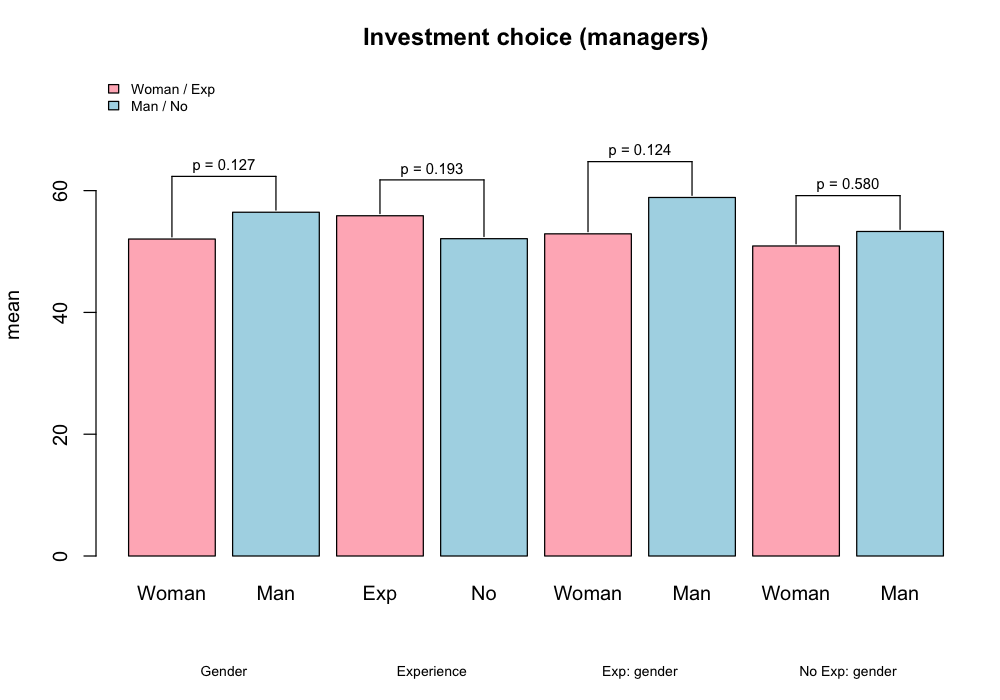
\includegraphics[scale=0.3]{../output/plots/invest_other_gender_experience} 
  \end{center}
    \caption{Delegated investment by gender}
  {\scriptsize Note:$p$-value is a t-test comparison between groups.  }
\end{figure}


\begin{result}\label{r2} Subjects tilt their portfolios and bid higher towards managers with experience, but split their portfolios equally and bid similarly between male and female managers given managerial experience. 
\end{result}


Table~\ref{tab:comparison} presents a comparison of shareholder choices, assessing managers' experience and gender in the different treatments. All shareholders first allocate their funds (1st stage) between managers, with or without experience. The allocation ratio, given the observed managerial choices, is predicted to be 1 because the state is drawn independently for each manager. We observe that allocation to the experienced (no experience) manager is 72 (28), making a ratio of 2.6 $>>$ 1.  

\begin{table}[hbtp]
  \caption{Choices by treatment}
  \label{tab:comparison}
  \footnotesize
  \begin{center}
    \begin{tabular}{lll|ll|ll|ll|ll|}
  \toprule
  & \multicolumn{2}{c}{1st stage} &  \multicolumn{2}{c}{T1} &  \multicolumn{2}{c}{T2} &  \multicolumn{2}{c}{T3} &  \multicolumn{2}{c}{T4}\\
  & Exp & No & M\_Exp & W\_exp & M\_exp & W\_no & W\_exp & M\_no & M\_no & W\_no   \\
  \midrule
\emph{Choices} & & & & &  & & & & &\\
Allocation & 72 & 28 & 51 & 49 & 68 & 32 & 71 & 29 & 49 & 51 \\
$p$-value & \multicolumn{2}{c|}{0.000} & \multicolumn{2}{c|}{0.816} & \multicolumn{2}{c|}{0.000} & \multicolumn{2}{c|}{0.000} & \multicolumn{2}{c|}{0.511}\\
Bid & 297 & 137 & 201 & 207 & 274 & 132 & 321 & 119 & 163 & 191 \\
$p$-value & \multicolumn{2}{c|}{0.000} & \multicolumn{2}{c|}{0.485} & \multicolumn{2}{c|}{0.000} & \multicolumn{2}{c|}{0.001} & \multicolumn{2}{c|}{0.284}\\
Price & 307 & 134 & 204 & 212 & 292 & 126 & 351 & 111 & 168 & 193 \\
$p$-value & \multicolumn{2}{c|}{0.000} & \multicolumn{2}{c|}{0.391} & \multicolumn{2}{c|}{0.000} & \multicolumn{2}{c|}{0.001} & \multicolumn{2}{c|}{0.376}\\
  \midrule
\emph{First order beliefs}  & & & & &  & & & & &\\
Investment & 119 & 82 & 125 & 123 & 118 & 76 & 134 & 85 & 99 & 98 \\
$p$-value & \multicolumn{2}{c|}{0.000} & \multicolumn{2}{c|}{0.745} & \multicolumn{2}{c|}{0.000} & \multicolumn{2}{c|}{0.000} & \multicolumn{2}{c|}{0.700}\\
Price & 336 & 214 & 279 & 276 & 328 & 186 & 364 & 163 & 210 & 234 \\
$p$-value & \multicolumn{2}{c|}{0.000} & \multicolumn{2}{c|}{0.618} & \multicolumn{2}{c|}{0.000} & \multicolumn{2}{c|}{0.000} & \multicolumn{2}{c|}{0.089}\\
  \midrule
\emph{Second order beliefs}  & & & & &  & & & & &\\
Investment & 122 & 81 & 124 & 121 & 124 & 79 & 134 & 79 & 93 & 92 \\
$p$-value & \multicolumn{2}{c|}{0.000} & \multicolumn{2}{c|}{0.444} & \multicolumn{2}{c|}{0.000} & \multicolumn{2}{c|}{0.000} & \multicolumn{2}{c|}{0.726}\\
Price & 349 & 216 & 279 & 270 & 344 & 179 & 373 & 158 & 214 & 230 \\
$p$-value & \multicolumn{2}{c|}{0.000} & \multicolumn{2}{c|}{0.266} & \multicolumn{2}{c|}{0.000} & \multicolumn{2}{c|}{0.000} & \multicolumn{2}{c|}{0.333}\\
  \midrule
\end{tabular}

  \end{center}
  {\scriptsize 
    Note: The $p$-value is the t-test comparison of choices between managers characteristis. 
    The test is performed at the group level for bid and prices, and at the invididual level 
    for the rest of the variables. 
  }
\end{table}

The tilt towards experienced managers is also evident in the treatments across columns T2 and T3, which differ in experience level and gender. In the former, the experienced (men) manager receives an allocation of 68\% and the no-experience (women) manager 32\%, or a ratio of 2.1. In the latter, the experienced (women) manager has 71\%, and the no-experience (men) manager has 29\%, which means a ratio of 2.5. In treatments with the same level of experience but different gender, the ratio is close to 1, meaning that subjects diversify as predicted: 51/49 (49/49) in T1 (T4) with experienced (no-experience) managers.

The bids follow the same behavior as in the allocation decisions. Market participants bid strongly for experienced managers. In the first stage, we observe a ratio of $297/137 = 2.2$. In T2, the ratio is $274/132 = 2.1$ while in T3 is $321/119 = 2.7$. When the managers have the same level of experience, the ratio is again closer to 1: 201/207 for T1 (all experience) and 163/191 for T4 (none with experience). The resulting market prices follow the behavior of bids, given that in the call market the price is the median bid. The price ratios are greater than 1 when comparing experience levels and closer to 1 when comparing managers with the same level of experience. 

\begin{result}\label{r3} The behavior observed in allocation and bid prices is consistent with the first- and second-order beliefs stated regarding managers' investment choices and share prices.
\end{result}

The second panel of Table~\ref{tab:comparison} presents subjects' first-order beliefs regarding investment and share prices. When comparing experience levels, subjects assess that the investment ratio (experience-over-no-experience investment beliefs) is much greater than 1, but when experience levels are fixed, the ratio equals 1. That is, the mechanism behind larger allocations and bid prices for experienced managers is driven by beliefs about investment choices. Looking at share price beliefs, the shareholders correctly anticipate market price behavior: a premium for experienced managers, but equal prices when the comparison keeps the same level of experience. 

As the correlation between first-order and second-order beliefs is strong\footnote{For the comparison in the first stage, the correlations are 0.85 for investment and 0.83 for price. For the other comparisons, the correlations are 0.79 for investment and 0.92 for price.} similar results appear when we analyze the second-order beliefs in the third panel of Table~\ref{tab:comparison}. The (belief) investment ratio is greater than 1 when comparing managers with dissimilar experience, but equal to 1 for the other cases. 



\begin{table}[!htbp]
  \centering
  \caption{Bid (log difference, OLS)}
  \label{tab:bid_reg}
  \footnotesize
  \begin{center}
      \begin{tabular}{l*{4}{c}}
    \toprule
     & \multicolumn{2}{c}{Exp $-$ No} & \multicolumn{2}{c}{ M $-$ W} \\
    \cmidrule(lr){2-3} \cmidrule(lr){4-5}
     & (1) & (2) & (3) & (4) \\
    \midrule
Woman & 0.147 & 0.171 & -0.002 & 0.076 \\
 & (0.116) & (0.113) & (0.130) & (0.123) \\
Investment belief (log diff) & 0.262** & 0.069 & -0.006 & -0.227 \\
 & (0.079) & (0.099) & (0.123) & (0.126) \\
Price belief (log diff) &  & 0.328** &  & 0.444*** \\
 &  & (0.106) &  & (0.096) \\
    \midrule
    Group fixed effects & Yes & Yes & Yes & Yes \\
    $N$ & 200 & 200 & 200 & 200 \\
    $R^2$ & 0.488 & 0.517 & 0.565 & 0.617 \\
    Adj. $R^2$ & 0.355 & 0.388 & 0.452 & 0.514 \\
    \bottomrule
  \end{tabular}

  \end{center}
    \begin{tablenotes}
  \footnotesize
  \item Note: all specifications include group FE. SE in parentheses. $^{*}p<0.05$, $^{**}p<0.01$, $^{***}p<0.001$.
  \end{tablenotes}
\end{table}


\begin{result} 
\label{r7}
There is no significant difference in the bids submitted by male and female subjects.
\end{result}




\end{document}